\documentclass{ctexart}

\usepackage[nea]{van-de-la-sehen}
\DeclareMathOperator*{\commentequals}{=\joinrel=\joinrel=\joinrel=}
\DeclareSIUnit{\stilb}{sb}
%\DeclareSIUnit{\steradian}{sr}
\usepackage{booktabs}

\begin{document}

\headerstamp

\subsubsection*{配置} % (fold)

\noindent
Reference Principle of Optics. Born, Wolf.\\
成绩: 平时40\%, 期末60\%, 小论文奖励.\\
每周五交作业, 每次2分.\\
随堂测验每次5分, (1-2次).\\
小论文参与则平时分加5, 得奖则+5/+4/+3. 1-3人每组.\\
平时分不超过40分.\\
Prof. Zhou Zongquan zq\_zhou@ustc.edu.cn\\
T.A. Qian Xing\\
T.A. Jin Xing\\
T.A. Jin Ming\\
考试时间2020年1月10日14:30\textasciitilde 16:30在5103和5102.

\centerline{
\begin{tabular}{|c|c|}
\hline
光线 & 反射, 折射 \\
\hline
波动 & 干涉, 衍射 \\
\hline
光子 & 光和物质相互作用  \\
\hline
\end{tabular}
}

% subsubsection 配置 (end)

\section{几何光学} % (fold)
\label{sec:几何光学}

\subsection{折射/反射定律} % (fold)
\label{sub:折射_反射定律}

\paragraph{组成物} % (fold)
\label{par:组成物}

\mbox{}
\centerline{
\begin{tabular}{|l|l|l|}
    \hline
    \+:r5{光线, 界面} & \+:r2{光线} & 发光点, 同心光束 \\
    \cline{3-3}
    & & 物和像 \\
    \cline{2-3}
    & \+:r3{界面} & 单个界面: 平面, 球面 \\
    \cline{3-3}
    & & 两个界面: 透镜 \\
    \cline{3-3}
    & & 多个界面: 透镜组 \\
    \hline
\end{tabular}
}

% paragraph 组成物 (end)

\paragraph{组成物间相互作用} % (fold)
\label{par:组成物间相互作用}

反射, 折射.

% paragraph 组成物间相互作用 (end)

\begin{finale}
    \begin{lemma}[反射/折射定律]
        绝对折射率: $n = c/v$, $n_{12} = n_2/n_1$.
        \[ n_1 \sin i_1 = n_2\sin i_2 \Rightarrow \frac{\sin i_1}{\sin i_2} = n_{12}. \]
    \end{lemma}
\end{finale}
\begin{remark}
    $n$大者谓光密集介质, 反之谓光疏介质.
\end{remark}
\begin{figure}[ht]
    \centering
    \incfig{6cm}{PointUnderWater}
    \caption{\cref{ex:折射水深}图}
\end{figure}
\begin{sample}
    \begin{ex}
        \label{ex:折射水深}
        图中
        \[ n_2\sin i = 1\cdot \sin i'. \]
        \[ y = \frac{x}{\tan i}, \]
        \[ y' = \frac{x}{\tan i'} = \frac{y\sqrt{1-n^2\sin^2 i}}{n\cos i}. \]
        $n$充分小时, $y' = y/n = 3/4$.
    \end{ex}
\end{sample}
\begin{figure}[ht]
    \centering
    \incfig{6cm}{SphericalRefr}
    \caption{\cref{ex:球面镜折射}图}
\end{figure}
\begin{sample}
    \begin{ex}
        \label{ex:球面镜折射}
        如图的球面镜, 构造$\rho' = nr/n'$, $\rho_2 = n'r/n$. 由SAS可得
        \[ \bigtriangleup MCH' \sim \bigtriangleup HCM. \]
        从而$i' = \varphi$, 从而
        \[ \frac{\sin \phi}{MC} = \frac{\sin i}{CH}. \]
    \end{ex}
\end{sample}
\begin{figure}[ht]
    \centering
    \incfig{6cm}{PlaneRefr}
    \caption{\cref{ex:平面折射}图}
\end{figure}
\begin{sample}
    \begin{ex}
        \label{ex:平面折射}
        按如图所示方法做图对平面折射显然可满足
        \[ n_1\sin i_1 = n_2\sin i_2. \]
    \end{ex}
\end{sample}
\begin{figure}[ht]
    \centering
    \incfig{6cm}{RefrAirport}
    \caption{\cref{ex:机场折射}图}
\end{figure}
\begin{sample}
    \begin{ex}
        \label{ex:机场折射}
        机场的折射率满足$n\pare{y} = n_0\pare{1+\beta y},$
        \[ n_0 = 1,\quad \theta_{max} = \pi/2. \]
        \[ \sin \theta_y = \frac{\rd{x}}{\sqrt{\rd{x}^2 + \rd{y}^2}} = \frac{n_0\sin\theta_0}{n_y}, \]
        \[ \+dxdy = \cot\theta_y = \frac{\sqrt{1-\sin^2\theta_y}}{\sin\theta_y} = \frac{\sqrt{n_y^2 - \pare{n_0\sin\theta_0}^2}}{n_0\sin\theta_0}. \]
        \[ \+dxdy \approx \sqrt{2\beta y} \Rightarrow x = \sqrt{\frac{2y}{\beta}}. \]
    \end{ex}
\end{sample}
\begin{finale}
    介质由$n_1$射入$n_2$的偏折量和由$n_1$射入$n'$再射入$n_2$的结果相同.
\end{finale}
\begin{lemma}[临界折射角]
    对于
    \[ i_c = \arcsin n_2/n_1, \]
    折射不再发生. 此时将发生全反射.
\end{lemma}
\begin{figure}[ht]
    \centering
    \incfig{6cm}{OpticalFibre}
    \caption{\cref{ex:光纤折射}图}
\end{figure}
\begin{sample}
    \begin{ex}
        \label{ex:光纤折射}
        光纤内有介质, 外有介质包裹. 其数值半径谓
        \[ \+r{N.A.} = n_0\sin\theta_0. \]
        其中$\theta_0$谓使其在$n_1$-$n_2$界面发生全反射的入射角度.
        \[ \begin{cases}
            n_0\sin\theta = n\sin\theta_1,\\
            n_1\sin\theta'_1 = n_2 \cdot 1.
        \end{cases} \Rightarrow \pare{\+r{N.A.}}^2 = n_1^2 - n_2^2. \]
    \end{ex}
\end{sample}
\begin{finale}
    进入折射率较大的介质时与法向夹角减小; 进入折射率较小的介质时反之增大并可能全反射.
\end{finale}
\begin{figure}[ht]
    \centering
    \incfig{8cm}{PoolRefr}
    \caption{\cref{ex:水池折射}图}
\end{figure}
\begin{sample}
    \begin{ex}
        \label{ex:水池折射}
        水池加水后, 水中物体的影像位置变化可能与其位置和观测者角度有关.
    \end{ex}
\end{sample}
\begin{pitfall}
    加入介质后像移动方向与物体位置相关.
\end{pitfall}
\begin{figure}[ht]
    \centering
    \incfig{6cm}{RefrPrism}
    \caption{\cref{ex:三棱镜偏转角}图}
\end{figure}
\begin{sample}
    \begin{ex}
        \label{ex:三棱镜偏转角}
        对于如图的三棱镜,
        \[ \delta = \pare{i_1-i_2} + \pare{i'_1 - i'_2}. \]
        \[ \alpha + \pare{\frac{\pi}{2} - i_2} + \pare{\frac{\pi}{2} - i'_2} = \pi \Rightarrow \alpha = i_2 + i'_2. \]
        最小偏转角$\delta$之条件谓$i_1 = i'_1$, $i_2 = i'_2$.
        \par
        此外, 由$n_0\sin i_1 = n\sin i_2$,
        \[ n_0 \sin \frac{\delta + \alpha}{2} = n\sin \frac{\alpha}{2}. \]
        \[ \boxed{n = n_0 \frac{\sin \pare{\alpha+\delta}/2}{\sin \alpha/2}.} \]
        故可以通过最小偏转角的测量得到介质折射率.
    \end{ex}
\end{sample}
\begin{remark}
    最小偏转角的条件$i_1 = i_2$和$i'_1=i'_2$可从$\rd{\delta} = \rd{\pare{i_1+i'_1}} = \rd{\pare{i_2+i'_2}}$可得$\rd{i_1} = -\rd{i'_1}$且$\rd{i_2} = -\rd{i'_2}$, 带入折射定律即可.
\end{remark}
\begin{remark}
    不同颜色光的出射角度不同(空间色散), 不同颜色光速度不同(时间色散).
\end{remark}
\begin{figure}[ht]
    \centering
    \incfig{10cm}{DropRainbow}
    \caption{彩虹的形成示意图}
    \label{fig:单色水滴折射}
\end{figure}
\begin{sample}
    \begin{ex}[彩虹的原理]
        \cref{fig:单色水滴折射}给出了单色光在水滴中折射的示意图, 有
        \[ D_f\pare{\alpha} = \pi + 2\alpha - 4\beta, \quad \frac{\sin \alpha}{\sin \beta} = n_f. \]
        $D_f\pare{\alpha}$对$\alpha$的关系在\cref{fig:水滴对不同入射角的偏折}中给出. 真正看到彩虹的地方是最小偏向角附近, 因为其光场能量最密集, 盖$D\pare{\alpha}$的任何微小偏离都可以覆盖相当大的$\alpha$区间. 此时
        \[ \alpha_m = \arccos\sqrt{\frac{n^2-1}{3}} \approx \SI{137.48}{\degree}. \]
        换言之, 应当在太阳光方向上方$\SI{42}{\degree}$寻找彩虹.
        \par
        虹经过两次折射一次反射, 霓经过两次反射两次折射. 后者入射的位置是水滴下方, 并且应当在太阳光方向上方$\SI{51}{\degree}$寻找之.
    \end{ex}
\end{sample}
\begin{figure}[htbp]
    \centering
    \includegraphics[trim={0 8cm 0 8cm},clip,width=8cm]{src/IncidentAlphaToDefl.pdf}
    \caption{水滴对不同入射角的偏折}
    \label{fig:水滴对不同入射角的偏折}
\end{figure}
\begin{theorem}[光路可逆]
    当光线方向反转时, 光将逆着同一路径传播.
\end{theorem}

% subsection 折射_反射定律 (end)

\subsection{Huygens原理} % (fold)
\label{sub:huygens原理}

\begin{figure}[ht]
    \centering
    \incfig{8cm}{Huygens}
    \caption{黑色为波线, 红色为波面, 蓝色的为次波}
    \label{fig:Huygens原理示意}
\end{figure}
\begin{definition}
    S波面上的每一面元是次波的波源. 次波源波面的包络是下一时刻的波面.
\end{definition}
\begin{sample}
    \begin{ex}
        如\cref{fig:Huygens原理示意}, Huygens原理可以正确解释球面波和平面波的传播.
    \end{ex}
\end{sample}
\begin{figure}[ht]
    \centering
    \incfig{8cm}{HuygensReflRefr}
    \caption{Huygens原理解释反射和折射定律}
    \label{fig:Huygens反射折射示意}
\end{figure}
\begin{sample}
    \begin{ex}[Huygens原理解释反射/折射定律]
        $A_nB_n = v_1 t$, $r_1 = v_1t$, $v_1t = A_1C_1$, 由是可得
        \[ i_1 = i'_1. \]
        折射定律中, $A_1B_n\sin i_2=A_1D_1 = v_2t$, $A_1B_n\sin i_1 = A_nB_n = v_1t$,
        \[ \frac{\sin i_1}{\sin i_2} = \frac{v_1}{v_2}. \]
    \end{ex}
\end{sample}
\paragraph{作业} % (fold)
\label{par:作业}

p.22-24: 1,3,4,7,11,12(p.16), p.32-33: 1,4,5(p.23), p.38-39: 1,2(p.27), taking dist Sun-Earth 1.5e8km, dist Moon-Earth 3.63-4.06e5km.

% paragraph 作业 (end)

% subsection huygens原理 (end)

\subsection{Fermat原理} % (fold)
\label{sub:fermat原理}

\begin{definition}
    光程即等价到相同时间内的真空传播距离.
    \[ \pare{QP} = \int_Q^P n\,\rd{l},\quad \tau_{QP} = \frac{\pare{QP}}{c}.  \]
\end{definition}
\begin{finale}
    \begin{theorem}[Fermat原理]
        两点之间光线传播的实际路径是使光程最短的路径.
    \end{theorem}
\end{finale}
\begin{figure}[ht]
    \centering
    \incfig{6cm}{MaxAndConstPathLen}
    \caption{光程取最大值和平稳值的示意}
    \label{fig:光程取最大值和平稳值的示意}
\end{figure}
\begin{sample}
    \begin{ex}
        光程并非总是最小值. 直线传播时是最小值, 球面镜一点到其对称点的反射是最大值, 椭圆镜是常值. 球面镜到对称点的光程实际上是
        \[ \sqrt{A+u} + \sqrt{A-u} \]
        的最值问题, 即$x^2+y^2=\const$的约束下求$x+y$的最值.
    \end{ex}
\end{sample}
\begin{figure}[ht]
    \centering
    \incfig{4cm}{FermatRefl}
    \caption{Fermat原理导出反射定律}
    \label{fig:Fermat原理导出反射定律}
\end{figure}
\begin{sample}
    \begin{ex}[Fermat原理蕴含反射定律]
        如\cref{fig:Fermat原理导出反射定律}, 显然入射角等于反射角的情形光程具有最小值.
    \end{ex}
\end{sample}
\begin{figure}[ht]
    \centering
    \incfig{8cm}{FermatRefr}
    \caption{Fermat原理导出折射定律}
    \label{fig:Fermat原理导出折射定律}
\end{figure}
\begin{sample}
    \begin{ex}[Fermat原理蕴含折射定律]
        $Q'M=x$, $MP' = p-x$,
        \begin{align*}
            \pare{QMP} &= n_1 QM + n_2 MP \\
            &= n_1\sqrt{h_1^2 + x^2} + n_2\sqrt{h_2^2 + \pare{p-x}^2}, \\
            \+dxd{\pare{QMP}} &= \frac{n_1 x}{\sqrt{h_1^2+x^2}} - \frac{n_2\pare{p-x}}{\sqrt{n_1^2+\pare{p-x}^2}} = 0 \Rightarrow \hfill\qed
        \end{align*}
    \end{ex}
\end{sample}

% subsection fermat原理 (end)

\subsection{成像} % (fold)
\label{sub:成像}

实发光点由能量产生, 而虚发光点无能量产生或经过, 仅仅视觉上光线发源. \emph{同心光束}谓光线本身或反向交于一点者.
\begin{figure}[ht]
    \centering
    \incfig{4cm}{ImaginaryEmit}
    \caption{虚发光点的例子}
    \label{fig:虚发光点的例子}
\end{figure}
\begin{sample}
    \begin{ex}
        如\cref{fig:虚发光点的例子}即为一虚发光点.
    \end{ex}
\end{sample}
\paragraph{物点和像点} % (fold)
\label{par:物点和像点}

光具组中的同心光束的交点分为物点和像点.
\begin{cenum}
    \item \emph{物点}: 若同心光束通过光具(组)前交于一点, 则谓该交点为物点.
    \begin{cenum}
        \item \emph{实物点}: 若交点为发出点, 则谓之实物点;
        \item \emph{虚物点}: 若(延长线)交点为汇聚点, 则谓之虚物点.
    \end{cenum}
    \item \emph{像点}: 若同心光束通过光具(组)后交于一点, 则谓该交点为像点.
    \begin{cenum}
        \item \emph{实像点}: 若交点为汇聚点, 则谓之实像点;
        \item \emph{虚像点}: 若(反向延长线的)交点为发出点, 则谓之虚像点.
    \end{cenum}
\end{cenum}

% paragraph 物点和像点 (end)
\begin{finale}
    实和虚以是否有能量区分之.
\end{finale}
\begin{longtable}{|c|c|c|}
    \hline
    \diagbox{物}{像} & 实像 & 虚像 \\
    \hline
    \+:r6{实物} & \+:r6{\incfig{4.5cm}{RealToReal}} & \+:r6{\incfig{4.5cm}{RealToIm}}\\
    &&\\
    &&\\
    &&\\
    &&\\
    &&\\
    光程 & $nQM + n'MQ'$ & $nQM - n'MQ'$ \\
    \hline
    \+:r6{虚物} & \+:r6{\incfig{4.5cm}{ImToReal}} & \+:r6{\incfig{4.5cm}{ImToIm}} \\
    &&\\
    &&\\
    &&\\
    &&\\
    &&\\
    光程 & $-nQM + n'MQ'$ & $-nQM - n'MQ'$ \\
    \hline
    \caption{实物/虚物成实像/虚像的例子}
    \label{table:实物虚物成实像虚像的例子}
\end{longtable}
\begin{sample}
    \begin{ex}
        \cref{table:实物虚物成实像虚像的例子}列举了实物/虚物成实像/虚像的例子.
    \end{ex}
\end{sample}

物点(包括实虚)构成之空间谓\emph{物方}, 像点(包括实虚)构成之空间谓\emph{像方}.
\begin{theorem}[物像共轭]
    一对物/像点和互换, 光路反向.
\end{theorem}
\begin{finale}
    \begin{theorem}
        \label{thm:物像等光程性}
        物点$Q$经过光具组反射/折射成像于点$Q'$, 则$Q$和$Q'$之间各条光线具有相等的光程.
    \end{theorem}
\end{finale}
\begin{pitfall}
    \cref{thm:物像等光程性}中物点/像点可能为实/虚, 但虚点的光程需要取反, 且虚物的光程取物方折射率, 虚像光程取像方折射率.\inlinehardlink{\cref{table:实物虚物成实像虚像的例子}}
\end{pitfall}
\begin{proof}
    考虑虚物成实像的例子,
    \[ \pare{\infty MQ} = \pare{\infty M} + \pare{MQ} = n\pare{\infty M + MQ} \]
    是光路无关的,
    \[ \pare{\infty MQ'} = \pare{\infty M} + \pare{MQ'} = n\infty M  + n'MQ \]
    也是光路无关的, 二者的差
    \[ \pare{QMQ'} = n'MQ - nMQ \]
    也是光路无关的.
\end{proof}
同心光束经过光具组变换后, 若能严格保持同心性, 则谓严格成像. 理想光具组谓是任意点严格成像者.
\begin{remark}
    真正的理想光具组仅有平面镜.
\end{remark}
\begin{lemma}
    只有等光程的反射/折射才能保证严格成像.
\end{lemma}
\begin{sample}
    \begin{ex}
        旋转椭球面为反射的等光程面.
    \end{ex}
\end{sample}
\begin{figure}[ht]
    \centering
    \begin{subfigure}{.45\textwidth}
        \centering
        \incfig{5cm}{EllipseRefl}
    \end{subfigure}
    \begin{subfigure}{.45\textwidth}
        \centering
        \incfig{5cm}{ParabolaRefl}
    \end{subfigure}
    \begin{subfigure}{.45\textwidth}
        \centering
        \incfig{5cm}{HyperbolaRefl}
    \end{subfigure}
    \begin{subfigure}{.45\textwidth}
        \centering
        \incfig{5cm}{PlaneRefl}
    \end{subfigure}
    \caption{反射等光程面}
\end{figure}
\begin{remark}
    Descartes椭球面是折射的等光程面.
\end{remark}
\begin{figure}[ht]
    \centering
    \incfig{6cm}{AplanaticSphere}
    \caption{齐明点}
    \label{fig:齐明点}
\end{figure}
\begin{sample}
    \begin{ex}[齐明点]\label{ex:齐明点}如\cref{fig:齐明点}寻找球面折射的等光程点,
        \[ QC = \frac{n'}{n}r,\quad Q'C = \frac{n}{n'}r \Rightarrow \bigtriangleup QMC \sim \bigtriangleup Q'MC, \]
        \[ \Rightarrow \frac{QM}{MQ'} = \frac{MC}{Q'C} = \frac{n'}{n}. \]
        \[ \boxed{n\pare{QM} - n'\pare{Q'M} = 0.} \]
    \end{ex}
\end{sample}
\begin{remark}
    直线传播(即平面波)严格而言在物理上不可能.
\end{remark}

% subsection 成像 (end)

\subsection{共轴球面组傍轴成像} % (fold)
\label{sub:共轴球面组傍轴成像}

\begin{figure}[ht]
    \centering
    \incfig{11cm}{RefrSingleSphere}
    \caption{单个球面折射示意}
    \label{fig:单个球面折射示意}
\end{figure}
\begin{proof}[单个球面的折射公式]
由折射定律,
\[ n\sin i = n'\sin i', \]
图中$\bigtriangleup CMQ$满足
\[ \frac{p}{\sin\phi} = \frac{s+r}{\sin i} = \frac{r}{\sin u} \Rightarrow \frac{p}{s+r} = \frac{\sin\phi}{\sin i}. \]
$\bigtriangleup CMQ'$满足
\[ \frac{p'}{\sin\phi} = \frac{s'-r}{\sin i'} = \frac{r}{\sin u'}\Rightarrow \frac{p'}{s-r} = \frac{n'}{n}\frac{p}{s+r}. \]
\[ \Rightarrow \frac{p}{n\pare{s+r}} = \frac{p'}{n'\pare{s-r}}. \]
平方之后代入余弦定理$\displaystyle \begin{cases}
    p^2 = s^2 + 4r\pare{s+r}\sin^2 \frac{\phi}{2},\\
    p'^2 = s^2 - 4r\pare{s'-r}\sin^2 \frac{\phi}{2},
\end{cases}$
\begin{equation}
    \label{eq:完整球面镜成像公式}
    \frac{s^2}{n^2\pare{s+r}^2} - \frac{s'^2}{n'^2\pare{s'-r}^2} = -4r\sin^2\frac{\phi}{2}\brac{\rec{n^2\pare{s+r}} + \rec{n'^2\pare{s'-r}}}. 
\end{equation}
\[ \phi\rightarrow 0\Rightarrow\frac{s^2}{n^2\pare{s+r}^2} = \frac{s'^2}{n'^2\pare{s'-r}^2} \Rightarrow \boxed{\frac{n'}{s'} + \frac{n}{s} = \frac{n'-n}{r}.} \qedhere \]
\end{proof}
\begin{remark}
    在\eqref{eq:完整球面镜成像公式}中令左右两侧同时为零, 可以得到一对共轭点, 无法严格成像.
\end{remark}
\begin{finale}
    \begin{remark}
        \eqref{eq:完整球面镜成像公式}只得到了一对共轭点. 绕球心旋转后可得到更多共轭点, 实际上是过这对共轭点垂直于光轴的平面.
    \end{remark}
\end{finale}
令$s'\rightarrow\infty$可得物方焦距
\[ s = f = \frac{nr}{n'-n}, \]
令$s\rightarrow\infty$可得像方焦距
\[ s' = f' = \frac{n'r}{n' - n}. \]
\begin{finale}
    \begin{theorem}[Gau\ss 公式]
        \[ \frac{f'}{s'} + \frac{f}{s} = 1,\quad f = \frac{nr}{n'-n},\quad f' = \frac{n'r}{n' - n}. \]
    \end{theorem}
\end{finale}
\setlength\extrarowheight{5pt}
\begin{table}[ht]
    \centering
        \begin{tabular}{|c|c|}
            \hline
            $s$ & 物点在球面左侧为正物距(实物)\\
            \hline
            \+:r2{$s'$} & 像点在球面右侧为正像距(实像) \\
            & 对于反射, 像在球面左侧为正, 右侧为负 \\
            \hline
            $r$ & 球心在球面右侧取正 \\
            \hline
            $u$ & 光轴到光线逆时针为正, 顺时针为负\\
            \hline
            $y$ & 光轴之上为正, 光轴之下为负 \\
            \hline
            $x$ & $Q$在$F$左侧为正, 右侧为负 \\
            \hline
            $x'$ & $Q'$在$F'$右侧为正, 左侧为负. \\
            \hline
        \end{tabular}
    \caption{符号约定}
    \label{table:符号约定}
\end{table}
\setlength\extrarowheight{0pt}
\begin{figure}[ht]
    \centering
    \begin{subfigure}{.3\textwidth}
        \centering
        \incfig{3cm}{SignConventionEx1}
        \caption{}
        \label{fig:符号约定示意1}
    \end{subfigure}
    \begin{subfigure}{.3\textwidth}
        \centering
        \incfig{3cm}{SignConventionEx2}
        \caption{}
        \label{fig:符号约定示意2}
    \end{subfigure}
    \begin{subfigure}{.3\textwidth}
        \centering
        \incfig{3cm}{SignConventionEx3}
        \caption{}
        \label{fig:符号约定示意3}
    \end{subfigure}
    \caption{符号约定示意}
    \label{fig:符号约定示意}
\end{figure}
\begin{sample}
    \begin{ex}
        \cref{fig:符号约定示意}中的三张图, 分别有符号
        \begin{cenum}
            \item 虚物$-s$, $-u$, 实像$s'$, $-u'$, 半径$+r$;
            \item 实物$s$, $u$, 虚像$-s'$, $u'$, 半径$-r$;
            \item 实物$s$, $u$, 虚像$-s'$, $u'$, 半径$+r$.
        \end{cenum}
    \end{ex}
\end{sample}
\begin{figure}[ht]
    \centering
    \incfig{10cm}{ReflSphere}
    \caption{球面反射成像示意}
\end{figure}
\begin{finale}
    \begin{theorem}[球面反射成像]
        \[ \rec{s'} + \rec{s} = \rec{f'},\quad f' = -\frac{r}{2}. \]
    \end{theorem}
\end{finale}
\begin{proof}
    由角平分线的性质, $\displaystyle \frac{AS}{AS'} = \frac{CS}{CS'} \Rightarrow \frac{s+r}{-\pare{r+s'}} = \frac{s}{s'}$.
\end{proof}
\begin{figure}[ht]
    \centering
    \begin{subfigure}{.9\textwidth}
        \centering
        \incfig{10cm}{RefrMagnification}
        \caption{折射球面镜的放大率示意图}
    \end{subfigure}
    \begin{subfigure}{.9\textwidth}
        \centering
        \incfig{10cm}{ReflMagnification}
        \caption{球面球面镜的放大率示意图}
    \end{subfigure}
    \caption{球面镜放大率}
    \label{fig:球面镜放大率}
\end{figure}
\begin{finale}
    \begin{theorem}[球面镜横向放大率公式]
        \label{thm:球面镜横向放大率公式}
        折射放大率为
        \[ \frac{y'}{y} = -\frac{ns'}{n's}. \]
        反射放大率为
        \[ \frac{y'}{y} = -\frac{s'}{s}. \]
    \end{theorem}
\end{finale}
\begin{proof}
    参考\cref{fig:球面镜放大率}, 对折射和反射的情形分别由有
    \[ \tan i = i = \frac{y}{s},\quad \tan i' = i' = \frac{-y'}{s},\quad ni = n'i'\Rightarrow \boxed{\frac{y'}{y} = -\frac{ns'}{n's},} \]
    \[ i' = i,\quad i' = -\frac{y'}{s},\quad \boxed{\frac{y'}{y} = -\frac{s'}{s}.} \qedhere \]
\end{proof}
在\cref{fig:单个球面折射示意}中, 考虑到$\displaystyle u = \frac{h}{s}$, $\displaystyle -u' = \frac{h}{s'}$, 可得
\begin{finale}
    \begin{theorem}[Lagrange-Helmholtz定理]
        \label{thm:Lagrange-Helmholtz定理}
        对多次由球面镜折射所得像,
        \[ ynu = y'n'u' = y''n''u''. \]
    \end{theorem}
\end{finale}

% subsection 共轴球面组傍轴成像 (end)

\subsection{薄透镜} % (fold)
\label{sub:薄透镜}

\paragraph{光焦度} % (fold)
\label{par:光焦度}

通常谓透镜的$\displaystyle\rec{f}$为其光焦度$p$(或$\Phi$), 但若物方和像方折射率不等, 即$n\neq n'$或$n,n'\neq 1$, 则$\displaystyle p = \frac{n'}{f'} = \frac{n}{f} = \frac{n'-n}{r}$.

% paragraph 光焦度 (end)

\begin{figure}[ht]
    \centering
    \incfig{10cm}{LensDualSphereImage}
    \caption{透镜成像示意}
    \label{fig:透镜成像示意}
\end{figure}
$d\ll r_1,r_2,s,s'$, $d\sim 0$, 对于面$\Sigma_1$,\\
\[ \frac{n}{s} + \frac{n_L}{s''} = \frac{n_L - n}{r_1} = \Phi_1. \]
对于面$\Sigma_2$, 考虑到$d \ll s''$,
\[ \frac{n_2}{-s''} + \frac{n'}{s'} = \frac{n'-n_L}{r_2} = \Phi_2. \]
其中$\Phi$表示光焦度, 从而
\[ \frac{n}{s} + \frac{n'}{s'} = \Phi_1 + \Phi_2 = \Phi = \frac{n_L - n}{r_1} + \frac{n'-n_L}{r_2}. \]
\begin{remark}
    这是\inlinehardlink{逐次成像法}的一个例子.
\end{remark}
\[ s' = \infty,\quad s = f = \frac{n}{\Phi}, \]
\[ s = \infty, \quad s = f' = \frac{n'}{\Phi}. \]
\begin{finale}
    \begin{theorem}[Gau\ss 物像公式]
        \begin{equation}
            \label{eq:Gauss物像公式}
            \frac{f'}{s'} + \frac{f}{s} = 1,\quad f = \frac{n}{\Phi},\quad f' = \frac{n'}{\Phi},\quad \Phi = \frac{n_L-n}{r_1} + \frac{n'-n_L}{r_2}. 
        \end{equation}
    \end{theorem}
\end{finale}
\begin{finale}
    \begin{theorem}[磨镜者公式]$n'=n\sim 1$时,
        \[ f = f' = \rec{\pare{n_L-1}\pare{\rec{r_1} - \rec{r_2}}}. \]
    \end{theorem}
\end{finale}
透镜视其对光的汇聚或发散作用可分为正透镜和负透镜,
\begin{cenum}
    \item $f>0$的透镜谓正透镜, 负值谓负透镜;
    \item 正透镜像方焦点在像方, 负透镜像方焦点在物方;
    \item 正透镜汇聚入射平行光, 负透镜发散之;
    \item {\color{red}空气中}, 中间厚, 边缘薄是正透镜; 反之为负透镜.
\end{cenum}
\begin{figure}[ht]
    \centering
    \begin{subfigure}{.45\textwidth}
        \centering
        \incfig{5cm}{PositiveLensSample}
        \caption{正透镜示意}
    \end{subfigure}
    \begin{subfigure}{.45\textwidth}
        \centering
        \incfig{5cm}{NegativeLensSample}
        \caption{负透镜示意}
    \end{subfigure}
    \caption{正负透镜示意}
\end{figure}
\begin{figure}[ht]
    \centering
    \incfig{10cm}{NewtonImage}
    \caption{Newton成像公式示意}
    \label{fig:Newton成像公式示意}
\end{figure}
如\cref{fig:Newton成像公式示意}, 代入\eqref{eq:Gauss物像公式}得
\[ \frac{f'}{f'+x'} + \frac{f}{f+x} = 1, \]
\[ xx' = ff'. \]
\begin{finale}
    \begin{theorem}[Newton成像公式]
        在\inlinehardlink{\cref{table:符号约定}}中的符号约定下,
        \begin{equation}
            \label{eq:Newton成像公式}
            xx' = ff'. 
        \end{equation}
    \end{theorem}
\end{finale}
由\inlinehardlink{\cref{thm:球面镜横向放大率公式}}, 参考\cref{fig:透镜成像示意}, 对透镜的两次成像(第二次为虚物成像)分别有(考虑到$d\rightarrow 0$)
\[ V_1 = -\frac{ns''}{n_L s},\quad V_2 = -\frac{n_Ls'}{n'\pare{-s''}}, \]
总放大率$V = V_1V_2$,
\begin{equation}
    \label{eq:FactorMagnification}
    V = -\frac{ns'}{n's} = -\frac{fs'}{f's} = -\frac{f}{x} = -\frac{x'}{f'} \commentequals^{f=f'}_{\text{i.e. }n=n'} -\frac{s'}{s} = -\frac{f}{x} = -\frac{x'}{f}. 
\end{equation}
\begin{finale}
    \begin{theorem}[透镜放大率公式]
        \[ V = -\frac{ns'}{n's}. \]
    \end{theorem}
\end{finale}
\begin{pitfall}
    对于一般透镜组, 放大率不可直接相乘.
\end{pitfall}
\begin{figure}[ht]
    \centering
    \incfig{6cm}{AirGlassAqLen}
    \caption{\cref{ex:空气玻璃水透镜}示意}
    \label{fig:空气玻璃水透镜示意}
\end{figure}
\begin{sample}
    \begin{ex}
        \label{ex:空气玻璃水透镜}
        等曲率双凸透镜, 放在水面上, 球面半径$\SI{3}{cm}$, 中心厚度$\SI{2}{cm}$, 玻璃和水的折射率分别为$1.50$和$1.33$, 透镜下$\SI{4}{cm}$物点$Q$, 计算曲面的光焦度, 并求$Q$点像的位置.
    \end{ex}
    \begin{proof}[解]
        光焦度直接套公式
        \[ \Phi_1 = \frac{n_g - n_a}{r_1},\quad \Phi_2 = \frac{n_0 - n_g}{r_2}, \]
        $\Sigma_1$成像
        \[ \frac{n_g}{s_1} + \frac{n_a}{s} = \Phi_1\Rightarrow s_1 = \SI{-0.054}{m}. \]
        $s_2 = 0.02 + 0.054 = \SI{0.074}{m}$, $\Sigma_2$成像
        \[ \frac{n_0}{s'} + \frac{n_g}{s_2} = \Phi_2\Rightarrow s' = -\SI{0.28}{m}. \]
        也就是在下方镜面下方$\SI{0.26}{m}$处.
    \end{proof}
\end{sample}
\begin{pitfall}
    非薄透镜不应当直接适用\eqref{eq:Gauss物像公式}.
\end{pitfall}

\paragraph{透镜组} % (fold)
\label{par:透镜组}

两个透镜符合的最简单情况,
\[ \rec{S'_1} + \rec{S_1} = \rec{f_1},\quad \rec{S'_2} + \rec{S_2} = \rec{f_2}. \]
两个透镜紧密接触, 则$S_2 = -S'_1$,
\[ \rec{s} + \rec{s'} = \rec{f_1} + \rec{f_2} = \Phi_1 + \Phi_2. \]

% paragraph 透镜组 (end)

\paragraph{作业} % (fold)
\label{par:作业}

p.38,39: 1, 2(p.27); p.55: 2, 4, 6, 8, 9(p.28).

% paragraph 作业 (end)

\paragraph{薄透镜做图法} % (fold)
\label{par:薄透镜做图法}

物方焦面和像方焦面谓而焦点处垂直于光轴之平面. \cref{fig:Newton成像公式示意}中两条竖直虚线分别表示物方焦面和像方焦面. 做图时满足性质
\begin{cenum}
    \setcounter{enumi}{-1}
    \item 入射平行线, 成像$F'$面;
    \item 入射平行于光轴的平行线, 出射过$F'$点;
    \item 入射过$F$点, 出射平行于光轴;
    \item 过透镜光心, 不变方向.
\end{cenum}
\begin{figure}[ht]
    \centering
    \incfig{8cm}{PositiveLenLines}
    \caption{正透镜做图示意}
    \label{fig:正透镜做图示意}
\end{figure}
\begin{figure}[ht]
    \centering
    \incfig{8cm}{NegativeLenLines}
    \caption{负透镜做图示意}
    \label{fig:负透镜做图示意}
\end{figure}
\begin{sample}
    \begin{ex}
        如\cref{fig:正透镜做图示意}和\cref{fig:负透镜做图示意}, 虽然分别是正透镜和负透镜, 但原理逐字句相同,
        \begin{cenum}
            \item 红色光线入射平行于光轴, 出射过$F'$; 橙色光线入射过$F$面, 故出射与之平行;
            \item 绿色光线过透镜光心, 出射不变方向; 青色光线入射与之平行, 故出射与之交于$F'$面;
            \item 紫色光线入射过$F$, 故出射平行于光轴; 蓝色光线入射与之平行, 故出射与之交于$F'$面.
        \end{cenum}
    \end{ex}
\end{sample}

% paragraph 薄透镜做图法 (end)

\paragraph{透镜组成像} % (fold)
\label{par:透镜组成像}

理想光具组将每个同心光束映射为同心光束. 其性质有
\begin{cenum}
    \item 点线面共轭对称到点线面;
    \item 光轴上的共轭点仍在光轴上;
    \item 垂直于光轴的平面, 共轭面垂直于光轴;
    \item 垂直于光轴同一平面内横向放大率相同;
    \item 不同平面内横向放大率一般不等, 但是只要有两个这样的平面横向放大率相等则横向放大率处处相等.
\end{cenum}
\begin{figure}[ht]
    \centering
    \begin{subfigure}{.95\textwidth}
        \centering
        \incfig{8cm}{UnionOfLens1}
        \caption{}
    \end{subfigure}
    \begin{subfigure}{.95\textwidth}
        \centering
        \incfig{8cm}{UnionOfLens2}
        \caption{}
    \end{subfigure}
    \caption{联合透镜成像}
    \label{fig:联合透镜成像}
\end{figure}
\begin{sample}
    \begin{ex}
        如\cref{fig:联合透镜成像}, 取二特殊光线作$L_1$所成像, 后以此像出发作$L_2$所成像.
    \end{ex}
\end{sample}

% paragraph 透镜组成像 (end)

\subsubsection{矩阵光学} % (fold)
\label{ssub:矩阵光学}

光线的特征用两个要素描述, 其方向与线上一点的位置. 方向定义为与主光轴的夹角, 用线上一点到主光轴的距离表示该点的位置. 光线经过球面后, 上述角度和高度的数值发生改变.\\
\begin{figure}[ht]
    \centering
    \incfig{8cm}{MatrixRefr}
    \caption{单球面的折射的反射}
\end{figure}
\[ i = \alpha + \pare{-\beta},\quad i' = \alpha' + \pare{-\beta}, \]
\[ \beta = \frac{y'}{x} = \frac{y}{x}, \]
\[ ni = n'i',\quad x\approx r\Rightarrow n\pare{\alpha + \frac{y}{x}} = n'\pare{\alpha' + \frac{y}{x}}, \]
\[ \begin{cases}
    n'\alpha' = n\alpha - \frac{n'-n}{r}y,\\
    y' = 0+y,
\end{cases} \]
\[ \Rightarrow \+vr = \begin{pmatrix}
    n\alpha\\
    y
\end{pmatrix}, \quad \+vr' = \begin{pmatrix}
    n'\alpha'\\
    y'
\end{pmatrix}, \quad \+vr' = R\+vr,\quad  R = \begin{pmatrix}
    1 & -\Phi \\
    0 & 1
\end{pmatrix}. \]
\begin{figure}[ht]
    \centering
    \incfig{8cm}{MatrixTrans}
    \caption{光线的传递矩阵}
\end{figure}
反射取$n'=n=-1$, $\Phi = -2/r$即可. 再考虑光传播的过渡矩阵,
\[ \+vr'_1 = \begin{pmatrix}
    n_1\alpha_1\\
    y'_1
\end{pmatrix},\quad \+vr_2 = \begin{pmatrix}
    n_2\alpha_2 \\
    y_2
\end{pmatrix}, \]
\[ y_2 = \alpha'_1 d_{21} + y'_1 = \alpha'_1n'_1\pare{\frac{d_{21}}{n'_1}} + y'_1, \]
\[ \+vr_2 = T_{21}\+vr_1,\quad T_{21} = \begin{pmatrix}
    1 & 0 \\
    \displaystyle\frac{d_{21}}{n'_1} & 1
\end{pmatrix}. \]
若再过$\Sigma_2$面, 结果为$\+vr_2$, 则最终
\[ \+vr' = R_2 T_{12} R_1 \+vr\Rightarrow \+vr' = S\+vr,\quad S = R_2 T_{21}R_1. \]
此处
\[ S = \begin{pmatrix}
    1 - \phi_2 d_{21}/n'_1 & -\pare{\Phi_1 + \Phi_2 - \Phi_1\Phi_2 d_{21}/n'_1} \\
    d_{21}/n'_1 & 1 - \Phi_1 d_{21}/n'_1
\end{pmatrix}. \]
设对于一一般透镜组, 其系统矩阵为$S$, 左右分别乘物到透镜组的过渡矩阵和像到透镜组的过渡矩阵得到总的物-像变换矩阵,
\begin{align*}
&S'= \begin{pmatrix}
    1 & 0 \\
    s'/m' & 1
\end{pmatrix}\begin{pmatrix}
    S_{11} & S_{12} \\
    S_{21} & S_{22}
\end{pmatrix}\begin{pmatrix}
    1 & 0 \\
    s/n_1 & 1 
\end{pmatrix}\\ &= \begin{pmatrix}
    S_{11} + \pare{s/n_1}S_{12} & S_{12} \\
    S_{21} + \pare{s/n_1}S_{22} + \pare{s'/n'_m}S_{11} + \pare{ss'/n_1n'_m}S_{12} & S_{22} + \pare{s'/n'_m}S_{12}
\end{pmatrix}.
\end{align*}
\[ y' = S'_{21}\pare{n\alpha} + S'_{22}\cdot y, \]
由于$y'$与$\alpha$无关, 故要求$S'_{21} = 0$. 这意味着
\begin{equation}
    \label{eq:物像位置关系}
    \boxed{\frac{s'}{n'_m} = -\frac{S_{21} + \pare{s/n_1}S_{22}}{S_{11}+\pare{s/n_1}S_{12}}.} 
\end{equation}
\begin{sample}
    \begin{ex}
        \cref{ex:空气玻璃水透镜}可以用矩阵光学的方法, 此时
        \begin{equation*}
        S = \begin{pmatrix}
            1 & -\Phi_2 \\
            0 & 1
        \end{pmatrix}\begin{pmatrix}
            1 & 0 \\
            d/n_g & 1
        \end{pmatrix}\begin{pmatrix}
            1 & -\Phi_1 \\
            0 & 1
        \end{pmatrix}
        = \begin{pmatrix}
            0.78 & -21.17 \\
            0.013 & 0.93
        \end{pmatrix}.
        \end{equation*}
        由\eqref{eq:物像位置关系}, 立刻有
        \[ s' = -\frac{\pare{s/n_1}S_{22}+S_{21}}{\pare{s/n_1S_{12}}+S_{11}} = \SI{-0.28}{\meter}. \]
    \end{ex}
\end{sample}
\paragraph{作业} % (fold)
\label{par:作业}

p69 2, 3, 8, 9, 11(p.49)

% paragraph 作业 (end)

% subsubsection 矩阵光学 (end)

% subsection 薄透镜 (end)

\subsection{理想光具组} % (fold)
\label{sub:理想光具组}

\begin{figure}
    \centering
    \incfig{8cm}{UnionOfLensAnalogLens2}
    \caption{理想光具组适用透镜规则}
    \label{fig:理想光具组适用透镜规则}
\end{figure}
如\cref{fig:理想光具组适用透镜规则}, 对于薄透镜适用的规则可直接迁移至理想光具组. 此外, Gau\ss 物像公式\eqref{eq:Gauss物像公式}和Newton成像公式\eqref{eq:Newton成像公式}仍然适用.
\par
基点谓光心, 基面谓二焦点所在面. $V=\pm 1$时构成主面.
\par
角放大率谓
\[ W = \frac{\tan u'}{\tan u}. \]
\begin{table}[hb]
    \begin{tabular}{|c|c|c|c|}
        \hline
        名称 & 定义 & 名称 & 定义\\
        \hline
        焦面 & 与无穷远平面共轭者 & 焦点 & 在光轴上者 \\
        \hline
        主面 & 横向放大率为$1$之共轭者 & 主点 & 在光轴上者 \\
        \hline
        & & 节点 & 角放大率为$1$之共轭者 \\
        \hline
    \end{tabular}
    \caption{光学点/面名词释义}
\end{table}
由于共轭主面的横向放大率为$1$, 任何方向射入透镜系统的光线都可以视为射入其中一主面后平行迁移至其共轭主面处后射出, 而方向准用薄透镜之规则.
\begin{figure}[htbp]
    \centering
    \begin{subfigure}{.4\textwidth}
        \centering
        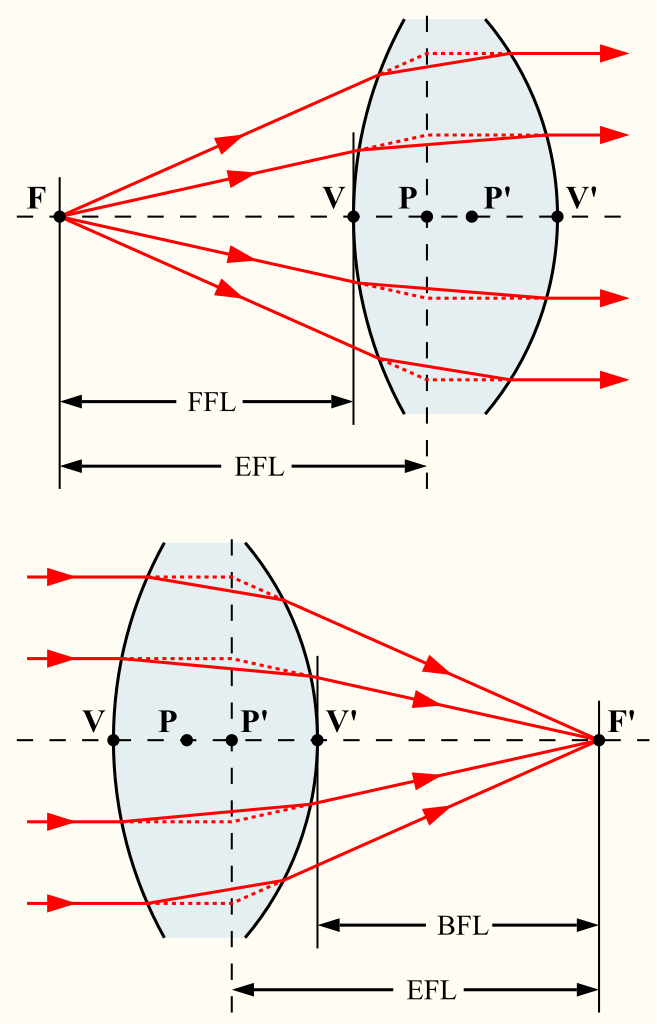
\includegraphics[width=\linewidth]{src/CardinalPoints.png}
        \caption{图中$P$为主点, 过其且垂直于光轴之平面为主面}
        \label{fig:主点示意图}
    \end{subfigure}
    \begin{subfigure}{.4\textwidth}
        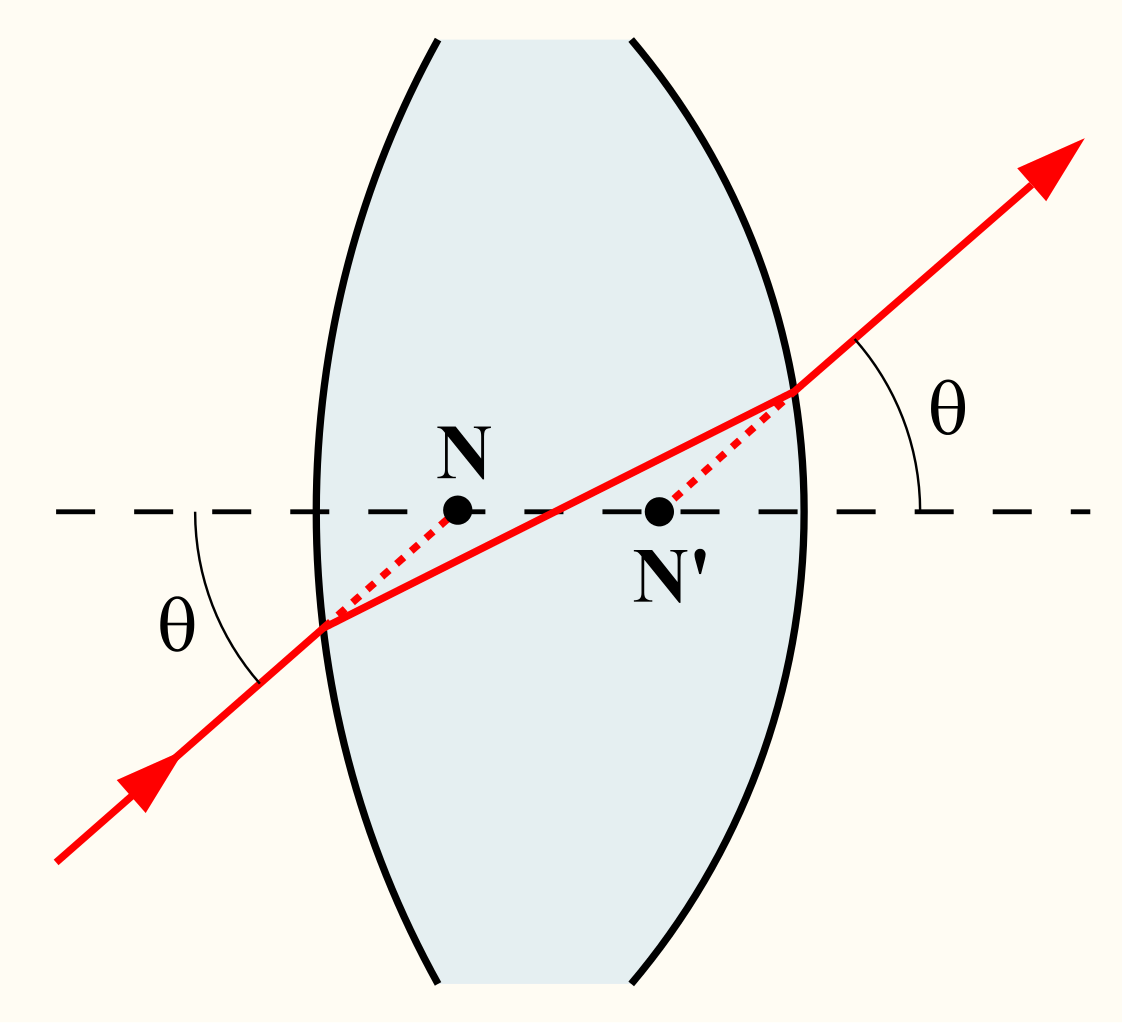
\includegraphics[width=\linewidth]{src/NodalPoints.png}
        \caption{节点示意图}
        \label{fig:节点示意图}
    \end{subfigure}
    \begin{subfigure}{.9\textwidth}
        \centering
        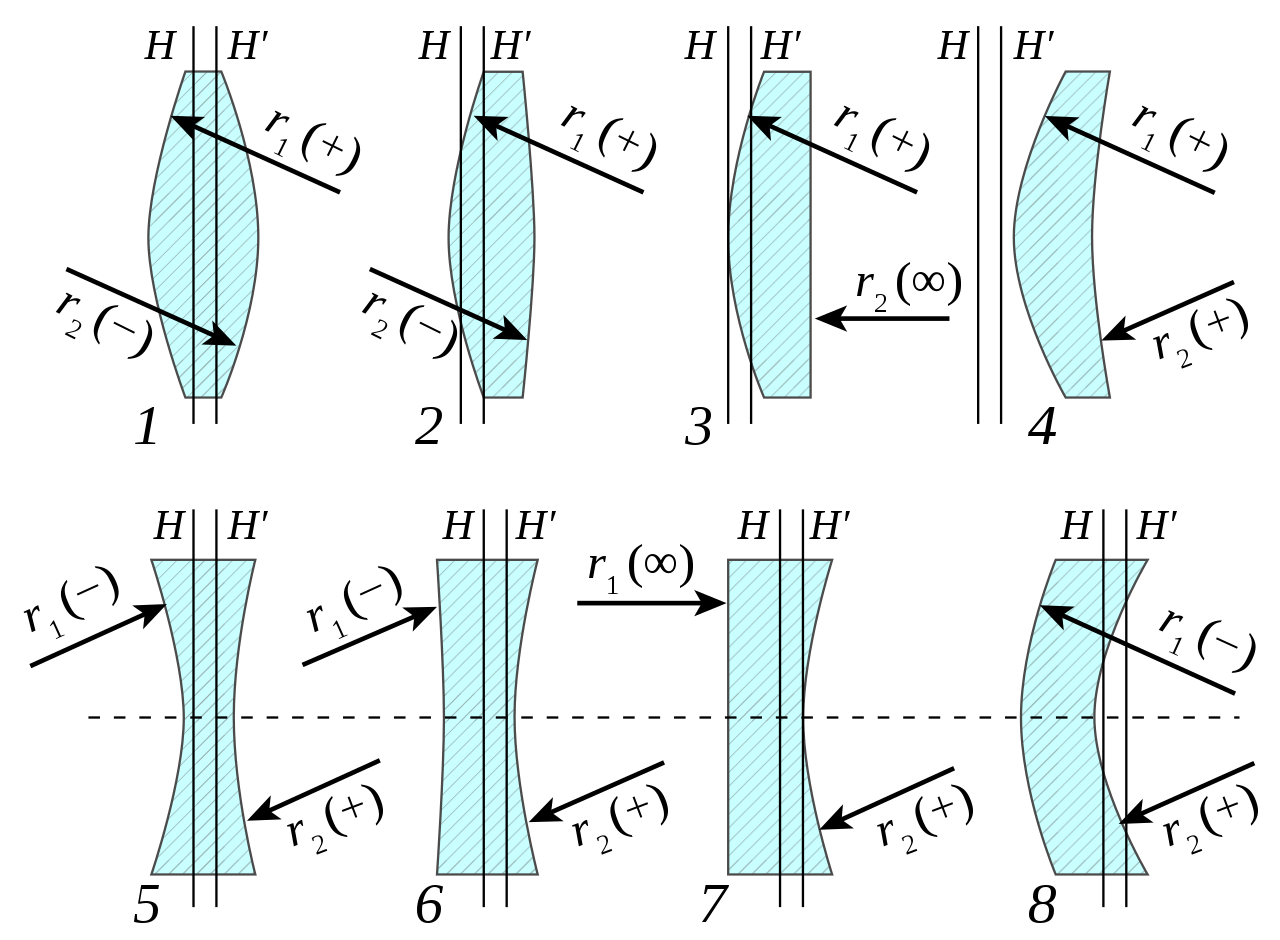
\includegraphics[width=\linewidth]{src/PrinciplePlanes.png}
        \caption{各种类型透镜的主面}
        \label{fig:各种类型透镜的主面}
    \end{subfigure}
    \caption{基面示意}
\end{figure}
\begin{figure}
    \centering
    \incfig{8cm}{PrinciplePlaneExample}
    \caption{主面示例}
    \label{fig:主面示例}
\end{figure}
\begin{sample}
    \begin{ex}
        如\cref{fig:主面示例}, 对给定物点先作出平行于光轴以及过物方焦点的直线, 将主面视为普通薄透镜后按一般法则成像即可.
    \end{ex}
\end{sample}
Gauss公式与Newton公式和横向放大率公式
\[ \frac{f'}{s'} + \frac{f}{s} = 1,\quad xx' = ff',\quad V = \frac{y'}{y} = - \frac{f}{x} = -\frac{fs'}{f's} \]
依然成立.
\begin{figure}
    \centering
    \incfig{8cm}{AngularFactor}
    \caption{角放大率示意}
    \label{fig:角放大率示意}
\end{figure}
如\cref{fig:角放大率示意}, 角放大率
\[ W = \frac{\tan u'}{\tan u} = -\frac{s}{s'} \Rightarrow VW = \frac{f}{f'}. \]
物方与像方折射率相等, 从而焦距相等时,
\[ f = f', \]
节点和主点重合.
\begin{theorem}[Helmholtz定理]
    \label{thm:Helmholtz定理}
    单个折射球面使空间所有点以任意宽广光束成像的必要条件为
    \[ yn\tan u = y'n'\tan u'. \]
\end{theorem}
在傍轴条件下, Helmholtz定理退化为\cref{thm:Lagrange-Helmholtz定理}.
\begin{figure}
    \centering
    \incfig{8cm}{UnionOfLens}
    \caption{理想光具组的联合}
    \label{fig:理想光具组的联合}
\end{figure}
确定系统的物方/像方焦点位置, 如\cref{fig:理想光具组的联合}, 对于平行入射光线, 作出过理想光具组出射光线与主光轴的交点, 即为联合后的(像方)焦点. 出射光线到达与入射光线等高处后即为(像方)主面. 物方沿相反方向确定即可.
\par
由几何关系立即得到
\[ x_H = \frac{f_1 d}{\Delta},\quad x'_H = \frac{f'_2 d}{\Delta}. \]
\[ f = -\frac{f_1f_2}{\Delta},\quad f' = -\frac{f'_1 f'_2}{\Delta}. \]

% subsection 理想光具组 (end)

\subsection{光学仪器} % (fold)
\label{sub:光学仪器}

\subsubsection{投影仪} % (fold)
\label{ssub:投影仪}

\begin{figure}[ht]
    \centering
    \incfig{10cm}{Projector}
    \caption{投影仪示意图}
    \label{fig:投影仪示意图}
\end{figure}
如\cref{fig:投影仪示意图}所示, 投影仪的工作原理如
\begin{cenum}
    \item 光源发出的光通过聚光镜后近似均匀地打在画片上;
    \item 画片处在投影镜头前$s\approx f$的位置;
    \item 画片的光通过投影镜头在屏幕上成像, 放大率
    \[ V = -\frac{s'}{s} \approx \frac{s'}{f}. \]
\end{cenum}

% subsubsection 投影仪 (end)

\subsubsection{照相机} % (fold)
\label{ssub:照相机}

\begin{figure}[ht]
    \centering
    \incfig{10cm}{Camera}
    \caption{照相机示意图}
    \label{fig:照相机示意图}
\end{figure}
如\cref{fig:照相机示意图}所示, 照相机的工作原理如
\begin{cenum}
    \item 物的距离$s$远大于焦距$f$;
    \item 感光片到镜头的距离$s'\approx f'$;
    \item 物经过镜头在感光片上成像.
\end{cenum}
\begin{figure}[ht]
    \centering
    \incfig{10cm}{CameraDof}
    \caption{景深示意图}
    \label{fig:景深示意图}
\end{figure}
如图, 由Newton公式, $xx' = ff'$, 从而
\[ \frac{\delta x'}{\delta x} = -\frac{f^2}{x^2}. \]
使得成像仍然清晰(光斑大小小于最小可分分辨距离)的$\delta x$谓景深. 当$x$足够大(物足够远时), 景深相应变大.

% subsubsection 照相机 (end)

\subsubsection{眼睛} % (fold)
\label{ssub:眼睛}

\begin{figure}[ht]
    \centering
    \incfig{8cm}{ShortSighted}
    \caption{人眼示意图}
    \label{fig:人眼示意图}
\end{figure}
如\cref{fig:人眼示意图}, 正常人眼的远点在无穷远处. 即从无穷远处发来的平行光将在视网膜处成像. 视网膜中央靠近光轴的一块小区域(黄斑)中具有最高的(物方)角分辨率, 白昼下大约为$1'$.
\par
眼睛的物/像方折射率不等, 从而二焦距不等, 主点和节点也不重合.

% subsubsection 眼睛 (end)

\subsubsection{放大镜和目镜} % (fold)
\label{ssub:放大镜和目镜}

\emph{视角放大率}谓通过仪器所称像所张角与肉眼所观察物体在明视距离处所成角之比
\[ M = \frac{w'}{w} \]
为视角放大率.
\begin{figure}[ht]
    \centering
    \incfig{10cm}{Magnify}
    \caption{放大镜示意图}
    \label{fig:放大镜示意图}
\end{figure}
如\cref{fig:放大镜示意图}, 在明视距离$s_0$以下虽然视角增加, 但眼睛不易观察. 通过将物体放在略近于放大镜焦点处, 可近似维持视角不变而在$s_0$外成像, 此时
\[ w' \approx \frac{y}{f} \Rightarrow M = \frac{w'}{w} \approx \frac{s_0}{f}. \]

% subsubsection 放大镜和目镜 (end)

\subsubsection{显微镜} % (fold)
\label{ssub:显微镜}

\begin{figure}[ht]
    \centering
    \incfig{10cm}{Micro}
    \caption{显微镜示意图}
    \label{fig:显微镜示意图}
\end{figure}
如图, 显微镜分两步成像.
\begin{cenum}
    \item 经过物镜成像, 大小$y_1$, 放大率由\eqref{eq:FactorMagnification}为
    \[ V_O = -\frac{\Delta}{f_O}. \]
    \item 经过放大镜(目镜)成虚像, 视角放大率为
    \[ M_E = \frac{s_O}{f_E}. \]
    \item 总的视角放大率为
    \[ \boxed{M = \frac{y_1/f_E}{y/s_0} = V_O M_E = -\frac{s_0\Delta}{f_Of_E}.} \]
\end{cenum}

% subsubsection 显微镜 (end)

\subsubsection{望远镜} % (fold)
\label{ssub:望远镜}

望远镜的视角放大率的定义为
\[ M = \frac{w'}{w}, \]
其中$w$远处物体在其位置上对眼睛的视角.
\begin{figure}[ht]
    \centering
    \incfig{10cm}{Tele}
    \caption{望远镜示意图}
    \label{fig:望远镜示意图}
\end{figure}
如\cref{fig:望远镜示意图}, 望远镜亦分为两步成像,
\begin{cenum}
    \item 物镜维持物体视角不变,
    \[ w = \frac{y}{f_O}. \]
    \item 目镜将视角放大为
    \[ w' = -\frac{y}{f_E}. \]
    总放大率为
    \[ M = \frac{w'}{w} = -\frac{f_O}{f_E}. \]
\end{cenum}
\begin{figure}[ht]
    \centering
    \incfig{10cm}{TeleGal}
    \caption{Galileo望远镜示意图}
    \label{fig:Galileo望远镜示意图}
\end{figure}
\cref{fig:Galileo望远镜示意图}中的望远镜则放大率为($f_E$取负数)
\[ w = \frac{y}{f_O},\quad w' = \frac{y}{-f_E}\Rightarrow M = \frac{w'}{w} = -\frac{f_O}{f_E}. \]
\begin{remark}
    望远镜实际通常使用反射式镜头以避免色差. 而此处所阐述者谓Kelper望远镜与Galileo望远镜.
\end{remark}

% subsubsection 望远镜 (end)

% subsection 光学仪器 (end)

\subsection{光阑} % (fold)
\label{sub:光阑}

\begin{figure}[ht]
    \centering
    \incfig{10cm}{Diaphragms}
    \caption{孔径光阑示意图}
    \label{fig:孔径光阑示意图}
\end{figure}
\begin{figure}[ht]
    \centering
    \incfig{10cm}{DiaphragmsWindows}
    \caption{视场光阑示意图}
    \label{fig:视场光阑示意图}
\end{figure}
\begin{cenum}
    \item \emph{光阑}谓对光具组成像是的光束孔径、成像点偏离光轴的范围加以限制的透镜边框、框架或特别设计的带孔屏障;
    \item \emph{孔径光阑}, 或\emph{有效光阑}, 谓真正确定通过光具组的光束孔径者;
    \item 被孔径光阑所限制之光束中边缘光线与物/像方夹角谓\emph{入射/出射孔径角};
    \item 孔径光阑在物方之共轭(可能是其本身)谓\emph{入射光瞳}; 在像方的共轭(可能是其本身)谓\emph{出射光瞳};
    \item 出射光瞳与入射光瞳之中心$O$和$O'$必定共轭. 通过轴外共轭点$P$, $P'$的光束过$O$, $O'$者谓\emph{主光线};
    \item 离光轴更远的共轭点之间的主光束可能被截断, 其边缘谓\emph{视场光阑};
    \item 通过视场光阑的光线中与光轴的夹角最大者谓\emph{入射/出射视场角}$w_0$和$w'_0$;
    \item 物平面上被$w_0$所限制者谓\emph{视场};
    \item 视场光阑在物方之共轭(可能是其本身)谓\emph{入射窗}; 在像方的共轭(可能是其本身)谓\emph{出射窗}.
\end{cenum}
当物点主见远离光轴, 即使离开视场外, 也可能成像. 只不过光线被截断者越来越多, 导致成像变暗, 即\emph{渐晕}.
\begin{pitfall}
    光阑是对于特定的共轭点而言的. 对于不同共轭点可以有不同光阑.
\end{pitfall}
如\cref{fig:孔径光阑示意图}, 中间的是孔径光阑, 左侧为入射光瞳, 右侧为出射光瞳. \cref{fig:视场光阑示意图}中实线为视场光阑, 虚线为光瞳. $P$发出的光线之一是主光线, $QP$即为视场半径.

% subsection 光阑 (end)

\subsection{像差} % (fold)
\label{sub:像差}

\begin{cenum}
    \item \emph{球差}谓轴上物点发出的大孔径光线不聚焦于一点之现象;
    \item \emph{彗差}谓轴外物点发出的宽光束不再交于一点, 形成状如彗星的亮斑;
    \item \emph{像散}谓水平方向和竖直方向的汇聚点(子午交线和弧矢交线)不在同一平面上; 二者某一处有光束为圆形, 谓\emph{明晰圈};
    \item 对于物平面上的所有点, 明晰圈有弯曲, 谓\emph{像场弯曲};
    \item \emph{畸变}谓横向放大率随$y$变化导致的放大率不一致;
    \item \emph{色差}谓折射率随频率改变导致不同颜色的光成像于不同地方且大小不同. 前者谓\emph{位置色差}, 后者谓\emph{放大率色差}.
\end{cenum}
\begin{ex}
    举例而言, 对于平行于对称轴的光线, 抛物面反射镜可以将光线完美地汇聚在一个点上. 然而方向相对于对称轴产生任何轻微的偏离后, 成像会发生彗差.
\end{ex}

\subsubsection{正弦条件} % (fold)
\label{ssub:正弦条件}

\paragraph{Abbe正弦条件} % (fold)
\label{par:abbe正弦条件}

这是光具组傍轴小物体以大孔径光束成像的条件.
\begin{figure}[ht]
    \centering
    \incfig{10cm}{AbbeSine}
    \caption{Abbe正弦条件示意图}
    \label{fig:abbe正弦条件示意图}
\end{figure}
如\cref{fig:abbe正弦条件示意图}, 成像时由Fermat原理知
\[ \pare{QMM'Q'} = \pare{QTT'Q'}, \quad \pare{PSS'F'} = \pare{QTTF'}, \]
\[ \pare{PNN'P'} = \pare{PSS'P'},\quad \pare{PNN'G'} = \pare{RMM'G'}. \]
傍轴条件下,
\[ \pare{F'Q'} = \pare{F'P'},\quad \pare{G'R'} = \pare{G'P'}. \]
由几何关系,
\begin{align*}
    & \phantom{ = } \pare{QMM'Q'} - \pare{RMM'G'}\\
    &= \pare{QR} + \pare{G'Q'} \\
    &= \pare{QTT'Q'} - \pare{PNN'G'} \\
    &= \pare{QTT'F'} + \pare{F'Q'} - \brac{\pare{PNN'P'} + \pare{P'G'}} \\
    &= \pare{QTT'F'} + \pare{F'Q'} - \brac{\pare{PSS'F'} + \pare{F'P'} + \pare{P'G'}} \\
    &= \pare{F'Q'} - \pare{F'P'} - \pare{P'G'}\\
    &= \pare{G'R'}.
\end{align*}
从而
\[ \pare{QR} + \pare{G'Q'} = \pare{G'R'}\Rightarrow \pare{QR} = \pare{Q'R'}, \]
\[ ny\sin u = n'y'\sin u'. \]
\begin{remark}
    Abbe正弦条件和\cref{thm:Helmholtz定理}(Helmholtz定理)不能同时成立.
\end{remark}
Abbe正弦条件可以理解为, 一个光学系统, 如果已经对轴上物点完美成像了, 那么想要对非常靠近光轴的物点也完美成像, 需要满足
\[ ny\sin u = n'y'\sin u'. \]
对于轴上点光源, 这要求光源发出的每一条傍轴光线都分别满足上面的式子. 对于平行光线, $y\sin u$正是其高度. 在这一条件下, 轻微偏离光轴的光线对于完美成像的偏离相对于这一条件不成立时是小量. \cref{ex:齐明点}中的齐明点满足这一条件. 事实上, 单一的球面折射面有三个齐明点, 另外两个分别为球心和球面上顶点.

% paragraph abbe正弦条件 (end)

% subsubsection 正弦条件 (end)

% subsection 像差 (end)

\subsection{光度学的基本概念} % (fold)
\label{sub:光度学的基本概念}

\paragraph{辐射能通量和光通量} % (fold)
\label{par:辐射能通量和光通量}

\emph{辐射能通量}, 或\emph{辐射功率}, 谓单位时间内光源发出或通过一定接收截面的辐射能, 记作$\Psi$. 若$\psi\pare{\lambda}$表示辐射能密度对波长的分布, 则
\[ \Psi = \int \psi\pare{\lambda}\,\rd{\lambda}, \]
其中$\psi$谓辐射能谱密度.
\par
对于人眼, 定义视见函数$V\pare{\lambda}$(明视觉)和$V'\pare{\lambda}$(暗视觉), $V\pare{\SI{555}{nm}} = 1$, 则\emph{光通量}
\[ \Phi = K_M \int V\pare{\lambda} \psi\pare{\lambda}\,\rd{\lambda}, \]
其单位为流明(lumen), 记作lm. 其中$K_M$是$\SI{555}{nm}$的光功当量.

% paragraph 辐射能通量和光通量 (end)


\paragraph{发光强度和亮度} % (fold)
\label{par:发光强度和亮度}

点光源沿某一方向的\emph{发光强度}谓该方向上单位立体角内的光通量.
\[ I = \+d{\Omega}d{\Phi}. \]
单位为candela, 记作cd.
\par
对于面光源, 面元朝向本身对光强有影响,
\[ B = \frac{\rd{\Phi}}{\rd{\Omega}\rd{S}\cos\theta} = \frac{\rd{I}}{\rd{S}\cos\theta} \]
为\emph{光度学亮度}, 其单位为$\SI{}{\lumen\per\square\meter\steradian}$, 或者
$\SI{}{\stilb} = \SI{}{\lumen\per\square\centi\meter\steradian}$, 其中$\theta$为面元法向与选定方向之夹角.
\par
将上式中的$\Phi$替换为$\Psi$分别得到\emph{辐射强度}和\emph{辐射亮度}.

% paragraph 发光强度和亮度 (end)

\paragraph{余弦发射体} % (fold)
\label{par:余弦发射体}

余弦发射体$\rd{I}\propto \cos\theta$, 定向发射体则如激光.

% paragraph 余弦发射体 (end)

\paragraph{照度} % (fold)
\label{par:照度}

\emph{照度}谓照射在单位面积上的光通量, 即
\[ E = \+d{S'}d{\Phi'}. \]
单位为Lux. 对于点光源,
\[ \rd{\Phi'} = I\,\rd{\Omega} = I\,\rd{S'}\,\cos\theta' / r^2\Rightarrow E = \frac{I\cos'}{r^2}. \]
对于面光源,
\[ \rd{\Phi'} = B\,\rd{\Omega}\,\rd{S}\,\cos\theta = \frac{B\,\rd{S}\,\rd{S'}\,\cos\theta\cos\theta'}{r^2}\Rightarrow E= \iint_S \frac{B\,\rd{S} \cos\theta\cos\theta'}{r^2}. \]

% paragraph 照度 (end)

\begin{table}[ht]
    \centering
    \begin{tabular}{>{\centering\arraybackslash}m{1.5cm}m{3cm}>{\centering\arraybackslash}m{3cm}>{\centering\arraybackslash}m{1cm}>{\centering\arraybackslash}m{1.2cm}}
        \toprule
        \+:c{1}{c}{术语} & \+:c{1}{c}{定义} & \+:c{1}{c}{定义式} & \+:c{1}{c}{符号} & \+:c{1}{c}{单位} \\
        \midrule
        辐射能谱密度 & 单位波长的辐射能通量 & $\displaystyle \rd{\Psi} = \psi\pare{\lambda}\,\rd{\lambda}$ & $\psi$ & $\SI{}{\watt\per\meter}$ \\
        \midrule
        辐射能通量/辐射功率 & 单位时间内光源发出或通过一定接收截面的辐射能 & $\displaystyle \Psi = \int \psi\pare{\lambda}\,\rd{\lambda}$ & $\Psi$ & $\SI{}{\watt}$ \\
        \midrule
        视见函数 & $\SI{5500}{\angstrom}$波长光与同感知亮度的$\lambda$波长光之$\Psi$比 & $\displaystyle V\pare{\lambda} = \frac{\Psi_{5500}}{\Psi_\lambda}$ & $V\pare{\lambda}$ & $\varnothing$ \\
        \midrule
        最大光功当量 & $\SI{5500}{\angstrom}$波长光的光功当量 & $K_M = \SI{683}{\lumen\per\watt}$ & $K_M$ & $\SI{}{\lumen\per\watt}$ \\
        \midrule
        光通量 & 经$V\pare{\lambda}$加权的$\Psi$ & $\displaystyle \Phi = K_M \int V\pare{\lambda}\psi\pare{\lambda}\,\rd{\lambda}$ & $\Phi$ & $\SI{}{\lumen}$ \\
        \midrule
        发光强度 & 点光源在某方向上单位单位立体角内发出的光通量 & $\displaystyle I = \+d\Omega dI$ & $I$ & $\SI{}{\candela}=\allowbreak\SI{}{\lumen\per\steradian}$ \\
        \midrule
        光度学亮度/亮度 & 面光源面元$\rd{S}$在某方向上单位投影面积$\rd{S^*}$的在该方向上的发光强度 & $\displaystyle B = \+d{S^*}dI \allowbreak= \+d{S\cos\theta}d{I}$ & $B$ & $\SI{}{\stilb}=\allowbreak\SI{}{\candela\per\square\centi\meter}$ \\
        \midrule
        照度 & 照射在单位面积上的光通量 & $\displaystyle E = \+d{S'}d{\Phi'}$ & $E$ & $\SI{}{\lux} = \allowbreak\SI{}{\lumen\per\square\meter}$ \\
        \bottomrule
    \end{tabular}
    \caption{光度学与辐射度学术语释义}
    \label{table:光度学与辐射度学术语释义}
\end{table}

\subsubsection{像的亮度, 照度与主观亮度} % (fold)
\label{ssub:像的亮度_照度与主观亮度}

对于余弦反射体, 反射亮度$B = \displaystyle \frac{E}{\pi}$.

\paragraph{像的亮度} % (fold)
\label{par:像的亮度}

像的亮度$B'$和物的亮度$B$之间成立$\displaystyle \frac{B'}{B} = k\pare{\frac{n'}{n}}^2$.

% paragraph 像的亮度 (end)

\paragraph{像的照度} % (fold)
\label{par:像的照度}

像平面上放置一屏幕, 则照度$E = k\pi B \displaystyle\pare{\frac{n'}{n}}^2u'^2_0 = \displaystyle \frac{k\pi B u_0^2}{V^2}$, 其中$V$为横向放大率, $k$为\emph{透光系数}. 傍轴近似下,
\[ E = k\pi B\pare{\frac{n'}{n}}^2 u'^2_0 = \frac{k\pi Bu_0^2}{V^2}. \]
\begin{ex}
    对于投影仪, 物方$u_0$几乎固定, 故物体放得越大, 亮度越小.
\end{ex}
\begin{ex}
    对于人眼和照相机, $u'_0$几乎固定,
    \[ u'_0 = \frac{D}{2f'} = \frac{n}{n'}\frac{D}{2f}, \]
    其中$D$为光阑直径. 故
    \[ E = \frac{k\pi B}{4}\pare{\frac{D}{f}}^2. \]
    相机上的$1,1.4,2,2.8,\cdots$就是$f/D$, 每次按$\sqrt{2}$倍增加, 故照度减少一半.
\end{ex}

% paragraph 像的照度 (end)

\paragraph{主观亮度} % (fold)
\label{par:主观亮度}

主观亮度谓单个视网膜细胞上的光通量. 天然主观亮度
\[ H_0 = E = \pare{\frac{n'}{n}}^2\frac{k\pi B}{4}\pare{\frac{D_e}{f_e}}^2, \]
其中$D_e$为瞳孔直径, $f_e$为眼睛焦距. 设$D'$为出射光瞳直径, 则望远镜$D' = D/M$, 显微镜$D'\propto \mathrm{N.A.}/M$, 其中$M$为视角放大率, $\mathrm{N.A.} = n\sin u_0$. 放大率充分大时, 上式中$D_e$应当用$D'$代替.

% paragraph 主观亮度 (end)

% subsubsection 像的亮度_照度与主观亮度 (end)

% subsection 光度学的基本概念 (end)

% section 几何光学 (end)

\paragraph{小论文选题} % (fold)
\label{par:小论文选题}

可自由选题, 参考如大气光学现象, 或像差矫正(显微镜, 天文望远镜).

% paragraph 小论文选题 (end)

\paragraph{作业} % (fold)
\label{par:作业}

p.97, 98 1, 2, 3, 6, 8 (p.70)

% paragraph 作业 (end)

\end{document}
